\documentclass[man]{apa6}

\usepackage{amssymb,amsmath}
\usepackage{ifxetex,ifluatex}
\usepackage{fixltx2e} % provides \textsubscript
\ifnum 0\ifxetex 1\fi\ifluatex 1\fi=0 % if pdftex
  \usepackage[T1]{fontenc}
  \usepackage[utf8]{inputenc}
\else % if luatex or xelatex
  \ifxetex
    \usepackage{mathspec}
    \usepackage{xltxtra,xunicode}
  \else
    \usepackage{fontspec}
  \fi
  \defaultfontfeatures{Mapping=tex-text,Scale=MatchLowercase}
  \newcommand{\euro}{€}
\fi
% use upquote if available, for straight quotes in verbatim environments
\IfFileExists{upquote.sty}{\usepackage{upquote}}{}
% use microtype if available
\IfFileExists{microtype.sty}{\usepackage{microtype}}{}

% Table formatting
\usepackage{longtable, booktabs}
\usepackage{lscape}
% \usepackage[counterclockwise]{rotating}   % Landscape page setup for large tables
\usepackage{multirow}		% Table styling
\usepackage{tabularx}		% Control Column width
\usepackage[flushleft]{threeparttable}	% Allows for three part tables with a specified notes section
\usepackage{threeparttablex}            % Lets threeparttable work with longtable

% Create new environments so endfloat can handle them
% \newenvironment{ltable}
%   {\begin{landscape}\begin{center}\begin{threeparttable}}
%   {\end{threeparttable}\end{center}\end{landscape}}

\newenvironment{lltable}
  {\begin{landscape}\begin{center}\begin{ThreePartTable}}
  {\end{ThreePartTable}\end{center}\end{landscape}}

  \usepackage{ifthen} % Only add declarations when endfloat package is loaded
  \ifthenelse{\equal{\string man}{\string man}}{%
   \DeclareDelayedFloatFlavor{ThreePartTable}{table} % Make endfloat play with longtable
   % \DeclareDelayedFloatFlavor{ltable}{table} % Make endfloat play with lscape
   \DeclareDelayedFloatFlavor{lltable}{table} % Make endfloat play with lscape & longtable
  }{}%



% The following enables adjusting longtable caption width to table width
% Solution found at http://golatex.de/longtable-mit-caption-so-breit-wie-die-tabelle-t15767.html
\makeatletter
\newcommand\LastLTentrywidth{1em}
\newlength\longtablewidth
\setlength{\longtablewidth}{1in}
\newcommand\getlongtablewidth{%
 \begingroup
  \ifcsname LT@\roman{LT@tables}\endcsname
  \global\longtablewidth=0pt
  \renewcommand\LT@entry[2]{\global\advance\longtablewidth by ##2\relax\gdef\LastLTentrywidth{##2}}%
  \@nameuse{LT@\roman{LT@tables}}%
  \fi
\endgroup}


  \usepackage{graphicx}
  \makeatletter
  \def\maxwidth{\ifdim\Gin@nat@width>\linewidth\linewidth\else\Gin@nat@width\fi}
  \def\maxheight{\ifdim\Gin@nat@height>\textheight\textheight\else\Gin@nat@height\fi}
  \makeatother
  % Scale images if necessary, so that they will not overflow the page
  % margins by default, and it is still possible to overwrite the defaults
  % using explicit options in \includegraphics[width, height, ...]{}
  \setkeys{Gin}{width=\maxwidth,height=\maxheight,keepaspectratio}
\ifxetex
  \usepackage[setpagesize=false, % page size defined by xetex
              unicode=false, % unicode breaks when used with xetex
              xetex]{hyperref}
\else
  \usepackage[unicode=true]{hyperref}
\fi
\hypersetup{breaklinks=true,
            pdfauthor={},
            pdftitle={The Development of Color Terms in Shipibo-Konibo Children},
            colorlinks=true,
            citecolor=blue,
            urlcolor=blue,
            linkcolor=black,
            pdfborder={0 0 0}}
\urlstyle{same}  % don't use monospace font for urls

\setlength{\parindent}{0pt}
%\setlength{\parskip}{0pt plus 0pt minus 0pt}

\setlength{\emergencystretch}{3em}  % prevent overfull lines


% Manuscript styling
\captionsetup{font=singlespacing,justification=justified}
\usepackage{csquotes}
\usepackage{upgreek}

 % Line numbering
  \usepackage{lineno}
  \linenumbers


\usepackage{tikz} % Variable definition to generate author note

% fix for \tightlist problem in pandoc 1.14
\providecommand{\tightlist}{%
  \setlength{\itemsep}{0pt}\setlength{\parskip}{0pt}}

% Essential manuscript parts
  \title{The Development of Color Terms in Shipibo-Konibo Children}

  \shorttitle{Color Terms in Shipibo-Konibo Children}


  \author{Danielle Kellier*\textsuperscript{1}, Martin Fortier*\textsuperscript{2}, Maria Fernández Flecha\textsuperscript{3}, \& Michael C. Frank\textsuperscript{4}}

  % \def\affdep{{"", "", "", ""}}%
  % \def\affcity{{"", "", "", ""}}%

  \affiliation{
    \vspace{0.5cm}
          \textsuperscript{1} University of Pennsylvania\\
          \textsuperscript{2} PSL Research University\\
          \textsuperscript{2} Pontificia Universidad Católica del Perú\\
          \textsuperscript{2} Stanford University  }

  \authornote{
    \begin{itemize}
    \tightlist
    \item
      these authors contributed equally.
    \end{itemize}
    
    Correspondence concerning this article should be addressed to Martin
    Fortier*, Postal address. E-mail:
    \href{mailto:my@email.com}{\nolinkurl{my@email.com}}
  }


  \abstract{Enter abstract here. Each new line herein must be indented, like this
line.}
  \keywords{keywords \\

    \indent Word count: X
  }





\usepackage{amsthm}
\newtheorem{theorem}{Theorem}[section]
\newtheorem{lemma}{Lemma}[section]
\theoremstyle{definition}
\newtheorem{definition}{Definition}[section]
\newtheorem{corollary}{Corollary}[section]
\newtheorem{proposition}{Proposition}[section]
\theoremstyle{definition}
\newtheorem{example}{Example}[section]
\theoremstyle{definition}
\newtheorem{exercise}{Exercise}[section]
\theoremstyle{remark}
\newtheorem*{remark}{Remark}
\newtheorem*{solution}{Solution}
\begin{document}

\maketitle

\setcounter{secnumdepth}{0}



\begin{verbatim}
## Warning: Unknown levels in `f`: agua, agua, agur, agna, agua, agur,
## amarillo, amarilla, amarillo, amarilla, amarillo, barin poi, barin poi,
## barrin poi, bavrinpui*, barri, bari, barri, barrinpui jisa, barin poi,
## blanco, blanco, blanco, carne, carne, carne, cheshe, chimapo, chimapo, emo,
## emo, espejo, espejokeska, jene, jene, jenekeska, jimi manxan, jimi manxan,
## jisa, jisa, joa, joa, joa, toshin, toshin, joshin metsashoko, joshinshama,
## joshinshama suki, joxo jakwokawa, joxo metsa, kasho, keskiti, koin,
## kononbi, konron, koro, libro, librokeska, mango, mango, mankoa, mankoa,
## mancoapei, mancoa pei, manxan yankon, manxan yankon, mierda sol, miarda,
## miarda del sol, miarda, miarda del sol, morada, morada, nai (lluvia), nai
## wiso, nai wisoa, naiwiso, naranjada, naranjado, narango, naranjo, anarando,
## narango, naranjada, naranjado, naranjo, negro, negro, negro, oxne,
## oxne, oxe, oxe, panshintani, panshinshima, panshinshima, pasto payota,
## pasto payota, pasto payota, pashnatani, andolni pei, pei panshin, pei
## panshinshoko, piel, piel, plomo, plomo, plomo, poa, ranchesh, rojo, rojo,
## roja, rojo, roja, rosa, rosa, rosa, ompash, unpasx, unpax, uva, uva color*,
## uva color, uva jisa, verdesito, verdesito, shokouerde, violeta, bioleta,
## violeta, bioleta, violeta, metsa shoko violeta, wisoshama, huiso, shane,
## shoo, yametani, yame wiso, yame wiso, yankontani, yakon, yakun, yankoncha,
## yakon, yakun, yankontani, yakonshama, yakunshama, yankon pasna, yankoncha,
## yancon, yankon joshin, yankon joshimansikaya, caña, cana, kaki, kaqui,
## pota, pota', nube, nuve, sero, serru, grub, grub, poi, manxanpui, manish,
## manish, oni, panshim oni, bari, barriwiso, chawa, chawa
\end{verbatim}

\begin{verbatim}
## Warning: Column `color_cat`/`Term (2017 survey)` joining factor and
## character vector, coercing into character vector
\end{verbatim}

\begin{verbatim}
## Warning: Unknown levels in `f`: agua, agua, agur, agna, agua, agur,
## amarillo, amarilla, amarillo, amarilla, amarillo, ambi, ambi, azul, azul,
## azu, azul, barin poi, barin pui, barrin pui, barrinpui, pui, barin poi,
## bavrinpui*, barri, bari, barri, barrinpui, barrinpui jisa, barin poi,
## bexnan, berrnan, bexna, bexnan, blanco, blanco, blanco, carne, carne,
## carne, celeste, celeste, celeste, chese, cheshe, chimapo, chimapu, chimapo,
## chocolate, chocolate, cielo, color cielo, cielo, coral, coral, emo, emu,
## emo, espejo, espejokeska, gris, gris, gris, jene, jene, jenekeska, jimi
## manshan, jisa, jisa, joxin, toshin, toshin, joshin metsashoko, joshinshama,
## joshinshama suki, joshin pasna, joshin pasna, joxo jakwokawa, joxo metsa,
## kari, cari, kari, karri, kasho, kashos, keskiti, kex keti, koin, kuin,
## kononbi, kunumbi, konron, korrum, kumrrum, kunrrum, koro, coro, coro,
## libro, librokeska, lila, lila, mango, mango, mankoa, mankoa, mancoapei,
## mancoa pei, manca, mandi, mandi, manrran, manxam, maxan, maxna, marron,
## marron, marron, maxe, maxe, mierda sol, miarda, miarda del sol, miarda,
## miarda del sol, morado, morado, morada, morado, morada, nia, nai (lluvia),
## nai wiso, nai wisoa, naiwiso, naranja, naranja, naranjada, naranjado,
## narango, naranjo, anaranjado, anarando, narango, naranja, naranjada,
## naranjado, naranjo, negro, negro, negro, nete, nete, oscuro, oscuro, oxne,
## oshne, oxne, oxe, oxe, panshintani, panshinshima, panshinshima, paxsna,
## pasto payota, pasto payota, pasto payota, parrna, pashnatani, paxna joshin,
## paxna joshin, andolni pei, pei panshin, pei panshinshoko, piel, piel,
## plomo, plomo, plomo, poa, pua, pua, ranchesh, ranchex, rojo, rojo, roja,
## rojo, roja, rosa, rosada, rosa, rosado, rosa, rosada, rosado, tena, tena,
## ompash, unpasx, unpax, uva, uva color*, uva color, uva jisa, verde, verde,
## cerde, verdesito, verde, verdesito, shokouerde, violeta, bioleta, violeta,
## bioleta, violeta, metsa shoko violeta, wisoshama, huiso, wiso yankon,
## wiso yankon, xena, xena, shane, xexi, shoo, rayame, yametani, rayanko,
## yankom, yankum, yankun, yankontani, yakon, yakun, yankoncha, yakon, yakun,
## yankontani, yankun, yakonshama, yakunshama, yankon pasna, yankoncha,
## yancon, yankon joshin, yankon joshimansikaya, caña, cana, kaki, kaqui,
## pota, pota', nube, nuve, sero, serru, grub, grub, poi, manxanpui, manish,
## manish, oni, panshim oni, bari, barriwiso, chawa, chawa
\end{verbatim}

\begin{verbatim}
## Warning in rbind(names(probs), probs_f): number of columns of result is not
## a multiple of vector length (arg 1)
\end{verbatim}

\begin{verbatim}
## Warning: 110 parsing failures.
## row # A tibble: 5 x 5 col     row col   expected  actual    file                        expected   <int> <chr> <chr>     <chr>     <chr>                       actual 1     1 <NA>  4 columns 8 columns '../data/WCS_Data/lang.txt' file 2     2 <NA>  4 columns 8 columns '../data/WCS_Data/lang.txt' row 3     3 <NA>  4 columns 8 columns '../data/WCS_Data/lang.txt' col 4     4 <NA>  4 columns 8 columns '../data/WCS_Data/lang.txt' expected 5     5 <NA>  4 columns 8 columns '../data/WCS_Data/lang.txt'
## ... ................. ... ............................................................. ........ ............................................................. ...... ............................................................. .... ............................................................. ... ............................................................. ... ............................................................. ........ .............................................................
## See problems(...) for more details.
\end{verbatim}

Color language is where language and perception meet. Terms like blue or
red draw boundary lines across a perceptually continuous space. In
English, there are 11 basic color terms, but this color categorization
is not universal. For instance, Russian speakers use two distinct words
to describe the colors light blue (\enquote{goluboy}) and dark blue
(\enquote{siniy}); and some languages have as few as two words (e.g.,
the Jalé people only have terms for \enquote{light} and \enquote{dark};
Berlin \& Kay, 1969). Why do languages vary in their color systems? One
emerging consensus is that languages categorize the color spectrum in
different ways in part due to functional demands (Gibson et al., 2017):
both smaller and larger color systems are relatively optimal for suiting
different communicative needs (Regier, Khetarpal, \& Kay, 2007).

One important component of this hypothesis is the idea that some color
systems are easier to learn for children than others; but the actual
acquisition of color terms -- while well-studied in English (e.g.,
Wagner, Dobkins, \& Barner, 2013) -- is extremely under-studied across
other populations. Berlin \& Kay's seminal World Color Survey (WCS;
Berlin \& Kay, 2009) presented adult speakers of over 100 languages with
differently colored chips and asked them to produce a label,
characterizing the space of color vocabulary in a range of written and
unwritten languages. The WCS is an invaluable resource for the
cross-linguistic study of color vocabulary, but no comparable resource
exists for cross-cultural studies of how this vocabulary is learned
across childhood.

In the current project, our goals were (1) to characterize color term
knowledge in an indigenous population previously studied by the WCS, the
Shipibo-Konibo (SK), and then (2) to build on this foundation to
characterize the developmental trajectory of color language acquisition
in a group of children raised learning Shipibo-Konibo, outside of the
WEIRD (Western Educated Industrialized Rich Democratic) populations that
are over-represented in behavioral science. Our approach here is to
begin by \ldots{}

\subsection{Color in Amazonian languages and Latin American varieties of
Spanish}\label{color-in-amazonian-languages-and-latin-american-varieties-of-spanish}

Only a handful of studies have explored the use of color terms in the
varieties of Spanish in Latin America. Berlin and Kay (1969) examine the
case of the Mexican dialect of Spanish, which they consider to be in
Stage VII of their classification (color systems in this stage, the most
advanced one, consist of between 8 and 11 color terms). According to
their proposal, there is a fixed evolutionary sequence of stages that
languages go through as they increase their color vocabulary; in this
sense, if a language encodes a category from a particular stage, it must
also encode those corresponding to all previous stages. They identify
the following basic color terms in t Mexican Spanish: blanco (white),
negro (black), rojo (red), verde (green), amarillo (yellow), azul
(blue), café (brown), morado (purple), rosa (pink), anaranjado (orange)
and gris (grey). Also, based on their work with forty Tzeltal
participants (, both Tzeltal monolinguals as well as Tzeltal-Spanish
bilinguals), they found that bilingualism did not skew their results
regarding the existence of semantic universals in the domain of color
vocabulary. Tzeltal has five basic color terms: ?ihk' (black), sak
(white), cah (red), ya (green) and k'an (yellow). This language is
estimated to be transitioning from Stage IV to V, which is reflected in
the ambiguity of the focus of yaš (grue). While all Tzeltal speakers
acknowledge that yaš includes two major perceptual centers (green and
blue), they vary in terms of their favored focal (either in the green or
blue area). The authors posit that a long history of contact with
Spanish has probably accentuated this, and suggest that exposure to
Spanish in schools will eventually cause yaš to be entirely restricted
to greens, and azul (or some other Spanish term) will be adopted into
the Tzeltal color system.

Mora Monroy (1989) offers information on Colombian Spanish based on
materials collected for the Linguistic-ethnographic Atlas of Colombia.
He presents examples of ad hoc color terms referring to colors through
objects prototypically instantiating these color: \enquote{vegetables},
\enquote{animals}, \enquote{food}, \enquote{metals}, \enquote{precious
stones}, \enquote{fire and its derivatives} and \enquote{atmospheric
phenomena}.

More recently, Aragón (2016) offers an ethnolinguistic study of color
terms in Mexican Spanish: amarillo (yellow), azul (blue), blanco
(white), café (brown, but literally \enquote{coffee}), gris (gray),
morado (purple), naranja (orange), negro (black), rojo (red), rosado
(pink) and verde (green). She analyzes the elaboration of these meanings
in dictionaries, as well as the references and associations to which
informants resort to for their own definitions. Aragón concludes that
the local natural and cultural referents constitute a point of consensus
among Mexicans when defining terms of color. Although informants also
discussed some cultural material referents, these were not salient
prototypes in their explanations. A special case that would merit
further study in the future is that of café in Mexico versus marrón in
Spain. According to the author, these two color terms are differentiated
by the prototype \enquote{toasted coffee grain} associated to the term
in Mexican Spanish. Finally, she reviews the symbolic associations
related to some terms, such as the discourses on femininity, especially
those centered around the figure of the girl, associated with the term
rosado.

Gibson et al. (2017) offer some approximations to the case of color
terms in Bolivian Spanish, based on their analysis centered on Tsimane,
an indigenous language spoken by a group living in the Amazonian
piedmont. The authors compare the Tsimane case with Bolivian Spanish and
American English. Compared to Bolivian Spanish and English, Tsimane
exhibits greater variability in terms of the color terms used for all
color chips presented in their study, with the exception of red. Out of
a total of 80 color chips, Tsimane exhibits 8 modal color terms while
English has 10, and Bolivian Spanish, 11. Also, despite the variability
observed, the assignment of modal color terms resulted in a similar
partition of the color space in the three languages assessed. The
authors also emphasize that the Tsimane color system is less informative
than the English and the Bolivian Spanish one. Finally, using the free
choice paradigm, they show speakers of Bolivian Spanish extensively use
the term verde (green) to denominate the color chips displayed, in
addition to celeste (light-blue) and azul (blue), as well as morado
(purple). Less frequent terms are, for example, fucsia (fuchsia), guinda
(maroon) and mostaza (mustard).

Several indigenous Amazonian color systems have been studied in the WCS.
One of them, Candoshi, has been further examined by Surrallés (2016). In
this thought-provoking study, Surrallés suggests that no proper color
term exists in this language. If the fieldworkers of the WCS found
otherwise, it is only because they misidentified the elicited terms as
color terms while they are nothing more than a series of ad hoc terms
referring to objects or animals of the surrounding environment. For
example, in Candoshi, the word for yellow is \enquote{ptsiyaromashi}
(\enquote{like the feathers of a milvago bird}), the word for red is
\enquote{chobiapi} (\enquote{ripe fruit}), the word for green is
\enquote{kamachpa} (\enquote{unripe fruit}), etc. These findings lead
Surrallés to argue that the Candoshi do not have a proper color system.
When they use \enquote{color terms} they are not trying to subsume
objects of the world under abstract color categories, but they are
rather establishing horizontal and ad hoc comparisons between similar
objects of the world.

In summary, while there is some dialect variation in Spanish\ldots{}

\subsection{The Development of Color
Vocabulary}\label{the-development-of-color-vocabulary}

To adult speakers, colors are extremely salient attributes of the
perceptual world; even when color is seemingly task-irrelevant, we
mention it (e.g., Sedivy, 2003). It is quite surprising then that
children often struggle to master color vocabulary. As reviewed by
Bornstein (1985), it has long been noted that color vocabulary is
learned quite late in development, with observations by Darwin, Bateman,
Nagel, and others attesting to individual children's delays in the
correct use of color terms well into middle childhood; several diarists
report 5 - 8 year olds with limited mastery of basic level color terms.
The age at which this difficulty is observed has been shifting over the
past hundred years, at least for English-speaking children, however.
Bornstein (1985) documents substantial decreases in the age at which
many children master the their colors, citing four years as an age at
which most children are proficient. Why Because colors are
cross-linguistically variable abstractions that are each part of a
broader system of concepts, children's acquisition of color vocabulary
has been an important case study for the \enquote{hard words} in
children's early language (Wagner et al., 2016).

This observation is even more interesting in light of the body of infant
research that suggests that infants' color discrimination abilities are
relatively well-developed by the end of the first year of life (for
review see e.g., Dobson \& Teller, 1978).

\subsection{The Current Study}\label{the-current-study}

In the last two decades, cross-cultural research aiming to go beyond
North-American \enquote{convenience samples} has mainly focused on the
study of East Asian children and adults. This endeavor has proved very
fruitful (Kitayama \& Cohen, 2007) but is still limited because of its
almost exclusive focus on North-American vs.~East-Asian samples. The
current study contributes to the general effort to go beyond such
samples and study the development of human cognition in a non-North
American and non-East Asian context. The SK people are an indigenous
group located within the Peruvian Amazon. They are mainly
horticulturalists, fishermen, occasionally hunters but are noted for
their strong display of tradition despite increasingly regular
interactions with the western world. Their children receive formal
schooling for 4 hours a day and begin formal Spanish lessons closer to
adolescence. Most SK adults have some grasp of Spanish but younger
adults show more proficiency than elders.

The SK indigenous people are particularly interesting for at least two
reasons: They differ from samples usually studied by cross-cultural
evolutionary psychologists (Apicella \& Barrett, 2016). Indeed,
evolutionary psychologists are particularly interested in the study of
contemporary hunter-gatherers because they are believed to a good model
of our Pleistocene ancestors. By contrast, like most riverine Amazonian
cultures, the SK culture is not based on hunting and gathering, but on
horticulture, fishing, and to a limited extent, hunting.

Because of their location on the Ucayali River, one of the main
tributaries of the Amazon, the SK culture has always been enmeshed in
rich trading networks involving other indigenous groups of the Andes and
the Lowlands (in pre-conquest times) as well as Mestizos and Westerners
(in post-conquest times) (Lathrap, 1970). It would thus be mistaken to
think of this culture as an \enquote{isolated} or \enquote{preserved}
one. On the contrary, having been extensively exposed to numerous
cultural influences, the SK culture has been constantly reworked and
reshaped through the centuries. This was especially true in the second
half of the 20th century with intense contact with the Spanish-speaking
Mestizo populations established along the Ucayali River. As a result,
today's SK culture straddles two worlds.

\section{Experiment 1}\label{experiment-1}

\begin{verbatim}
## Warning in evalq(as.numeric(as.character(edad)), <environment>): NAs
## introduced by coercion
\end{verbatim}

\subsection{Methods}\label{methods}

\subsubsection{Participants}\label{participants}

We recruited 39 adult participants (7 men). Most of participants were
from SK communities of the Middle Ucayali region (from Yarinacocha, San
Francisco, and Nueva Betania), but some of them were from communities of
the Lower (Paoyhan) and Upper (Puerto Belen) Ucayali. In Yarinacocha (a
small town located in the vicinity of Pucallpa), participants were
recruited in Bena Jema, a neighborhood where most of the inhabitants are
SK. All the other places where participants were recruited were native
community villages exclusively inhabited by SK people. Overall, the
sample included both somewhat urbanized SK (Yarinacocha and San
Francisco) and SK still used to more traditional activities and regular
contact with the surrounding rainforest (Nueva Betania, Paoyhan, and
Puerto Belen). \ldots{}. The median age for participants was roughly 38
years with a range between 20 to 64 years of age (SD = 13.60yo).
Regarding occupations, 41\% of the women were homemakers (33\% overall)
and another 41\% were artisans (33\%).
\texttt{tools::toTitleCase(as.character(as.english(filter(study1\_occupations,\ género\ ==\ \textquotesingle{}masculino\textquotesingle{}\ \&\ ocupación\ ==\ \textquotesingle{}agricultor\textquotesingle{})\$n)))}
of the 7 men were horticulturalists (43\%, 8\% overall). Four women
(12\%, 10\% overall) and three men (43\%, 8\% overall) identified as
students. Although all adult participants spoke Shipibo-Konibo as a
first language, all started learning Spanish before early adolescence
(median = 8yo, SD = 2.90y).

\subsection{Materials}\label{materials}

The stimuli that were used for this study included 330 color chips.
However, only 165 chips were used for each single participant (see
below). These chips were exactly those that were used to collect the
data of the WCS. The 330 hues of the set of chips can be visualized in
Appendix 1. Dimensions of the chips are 2 cm x 2.5 cm.

\subsection{Procedure}\label{procedure}

The procedure was similar to that used in the WCS (see Berlin \& Kay
2009: 585-591), but it differed in some respects. Participants were
seating in front of the experimenter. In order to make sure that the
natural light intensity would not vary much between participants, the
experiment was taking place indoors, near a window or a door. The study
was conducted in SK language.

Participants were first introduced to the whole procedure and the
general goal of the study. They were next presented with a color chip
and being asked: \enquote{What is the color of this chip?}. (Note that
the SK word for color that we used was the Spanish word color. Indeed,
the SK language includes some castillanisms -- that are well-known by
all speakers --, and color is one of them.)

A difference between the WCS procedure and ours is that, in the WCS, the
experimenter was expected to brief participants so that they would only
provide basic color terms during the task (e.g., \enquote{blue} as
opposed to \enquote{navy blue} or \enquote{sky-like}). However, we found
it rather difficult to make participants grasp in a few sentences what a
basic color term is.\^{}{[}Indeed, as Berlin \& Kay (2009: 587-589)
acknowledge, there is no straightforward necessary and sufficient
criteria for the \enquote{basicness} of a color term.\} This is why we
decided to let participants provide any term they wished, but, when they
were not providing a basic color term, we would ask further questions to
eventually elicit a basic color term. For example, if, when presented
with a red color chip, the participant was providing the term
\enquote{blood-like} (a non-basic color term), the experimenter would
ask: \enquote{Do you know of any other word to refer to the color of
this chip?} If the participant subsequently responded \enquote{dark red}
(another non-basic color term), the experimenter would further ask:
\enquote{How would you refer to this color with only one word?}.
Eventually, the participant would say: \enquote{red} (a basic color
term). For some chips, participants would provide a basic color term at
once; but for others, they would first provide one or two non-basic
terms before actually providing a basic term. When participants did not
provide a basic color term after three trials (i.e., two follow-up
questions), no further questions was asked, and the experimenter was
moving to the next chip. Admittedly, proceeding this way proved more
effortful and time-consuming than the WCS procedure, but it improved the
fluency and the intuitiveness of the task for participants.

Another difference between our procedure and that of the WCS concerned
the number of chips each single participant was presented with. In the
WCS, every participant was expected to provide color terms for each of
the 330 chips of the set. As we were afraid that doing so would take too
long and that participants would find the task exceedingly tedious, we
decided that the set of chips would be split in two (even and uneven
numbers) and that every participant would be randomly ascribed to one of
the two subsets. As a result, each participant was presented with only
165 chips.

\subsection{Results and Discussion}\label{results-and-discussion}

All participants described at least 1 chip with the following set of
color terms: light/white (\enquote{joxo}), dark/black (\enquote{wiso}),
yellow (\enquote{panshin}), red (\enquote{joshin}), and green/blue
(\enquote{yankon}). Most (79\%) participants also used described at
least 1 chip as faded or \enquote{manxan}, referring to a chip's
saturation. In terms of overall popularity, participants on average
described 32\% of chips as \enquote{yankon} (\emph{SD} = 10\%) followed
by \enquote{joshin} (\emph{M} = 12\%, \emph{SD} = 6\%), \enquote{joxo}
(10\%, 5\%), \enquote{panshin} (9\%, 4\%), \enquote{manxan} (7\%, 7\%),
and \enquote{wiso} (6\%, 4\%).

One departure from the Berlin-Kay data was that 59\% of adults described
at least 1 chip using a Spanish-language color term, accounting for 4\%
of all responses (Figure 1a-b). In particular, spanish use reached as
high as 55\% when participants were asked to label chips that English
speakers would consider to be orange. However, there was a high amount
of variability in Spanish use between subjects (\emph{M} = 4\%,
\emph{SD} = 12\%) with some subjects never responding in Spanish. One
responded in Spanish for 0\% of all trials despite all sessions being
conducted entirely in the Shipibo-Konibo language.

Participants on average described 69\% of chips using a SK-language
basic color term like \enquote{yankon} (\emph{SD} = 22\%). Some
participants described chips using SK-language ad hoc color terms, such
as \enquote{nai} or \emph{sky} for blue chips (\emph{M} = 11\%,
\emph{SD} = 12\%), or ad hoc terms referring to saturation or luminosity
of a chip, such as \enquote{manxan} (\emph{M} = 7\%, \emph{SD} = 7\%).
Virtually all instances where a participant responded in Spanish
involved a Spanish basic color term such as \enquote{rojo} (\emph{M} =
4\%, \emph{SD} = 10\%). In other words, participants only responded in
Spanish to label chips into basic categories but relied on
Shipibo-Konibo all other descriptor types.

\textbf{Gender differences in term profusion or term appearance}

We speculated as to whether or not there were overall gender differences
in responses given during Study 1, especially considering the
differences in reported occupations across genders. We found no
significant differences in the overall spread of color term usage across
the set (\emph{t} = 0, \emph{P} = 1) or in the percentage of subjects
who used a term at least once throughout the task (\emph{t} = -0.38,
\emph{P} = 0.71).

\textbf{Entropy analyses}

\begin{figure}
\centering
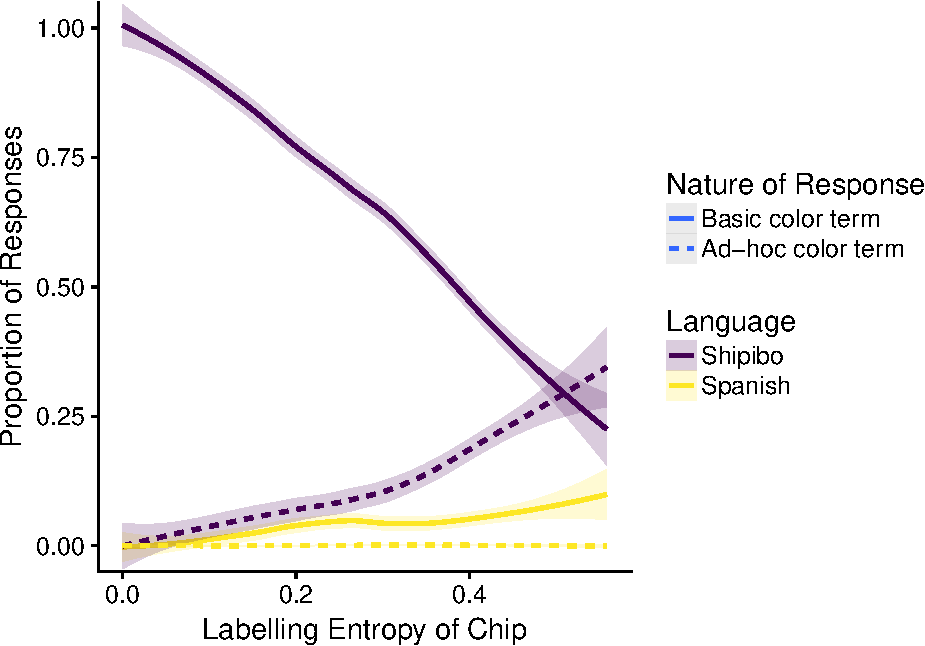
\includegraphics{amazon_color_files/figure-latex/study1_entropyanalyses-1.pdf}
\caption{}
\end{figure}

\section{Experiment 2}\label{experiment-2}

In Study 2, we tested children on their production and comprehension
skills with a set of chips representing the prototypical colors for
common Shipibo terms.

\subsection{Methods}\label{methods-1}

\subsubsection{Participants}\label{participants-1}

The Pontificia Universidad Católica del Perú's Institutional Review
Board approved our study protocol. We recruited 57 5- to 11-year-old
children (23 boys). Table 1 details the distribution of age and gender.
Fifteen children were recruited from neighborhoods in Yarinacocha, in
the Pucallpa region of Peru, as well as in 42 children from Bawanisho, a
native community settled along the Ucayali River, south of Pucallpa.
Children were recruited either through their parents or through local
schools. When recruited at school, consent for participation was
collected from both the teachers and the parents; otherwise, only
consent from the parents was collected.

\subsubsection{Materials}\label{materials-1}

Based on findings of Study 1, we singled out 8 color chips that were
prototypical instances of prominent SK color terms. These color chips
were blue (WCS n°1), green (WCS n°234), red (WCS n°245), white (WCS
n°274), yellow (WCS n°297), black (WCS n°312), greeny-yellow (WCS
n°320), and purple (WCS n°325). (To visualize the hue of these chips,
see Appendix 1.) These color chips were exactly the same as those used
in Study 1; the only difference was that while 330 chips were used in
Study 1, only 8 of them were used in Study 2.

\subsubsection{Procedure}\label{procedure-1}

The production and comprehension tasks were both conducted in SK. In
both tasks, children were seating in front of the experimenter; a table
(on which the color chips were displayed) was standing between them. For
obvious reasons, the production task was always performed before the
comprehension task. Production task. The procedure was very similar to
that of Study 1. Children were first introduced to the whole procedure
and the general goal of the study. It was specified that they would be
expected to provide color terms in SK (and not in Spanish). Children
were then asked: \enquote{What is the color of this chip?}. As with
adults, we used follow-up questions to elicit basic color terms when
terms initially provided were not basic. When children provided Spanish
color terms, the experimenter would write down their response but
further ask: \enquote{What is the name of this color in SK?}. When
children were replying \enquote{I don't know} to this prompt, the
experimenter would not ask further questions and would move forward to
the next color chip. As a result, responses of some children include
only non-basic SK color terms or Spanish color terms. In total, we
collected production data for 8 color chips. For each chip, the data
include either one response (when children provided a SK basic color
term in the first trial) or two or three responses (when children's
initial responses were either non-basic and/or in Spanish).

Comprehension task. The procedure of the comprehension task was quite
different. The aim of this task was to examine how good children were at
understanding the meaning of color terms. The 8 color chips of the
production task were simultaneously displayed in front of the children.
The experimenter would then ask: \enquote{Can you give me the \_\_\_
chip?} (where ``\_\_\_'' stands for a color term). In total, the
comprehension of 9 SK color terms was tested. The choice of these terms
was based on the findings of Study 1. Not all of them were basic, but
all of them stood out as being prominent in the SK color system. The 9
terms used as prompts included: yankon (\enquote{grue}), joshin
(\enquote{red}), panshin (\enquote{yellow}), joxo (``white), wiso
(\enquote{black}), nai (\enquote{blue}), and barin poi
(\enquote{greeny-yellow}); in addition, as Study 1 revealed that two
non-basic terms are widely used to refer to green and purple, two words
were used to test comprehension of each of these two colors: pei/xo
(\enquote{green}) et ami/pua (\enquote{purple}). Furthermore, Study 1
showed that for some of these color terms, only one response was
accurate, while for others, several responses were equally correct. For
example, only one chip could be picked up as an instance of wiso. By
contrast, four chips could be considered to be instances of yankon
(blue, green, greeny-yellow, and, to a lesser extent, purple); two chips
for joshin (red, and, to a lesser extent, purple); and two as well for
pei/xo (green, and, to a lesser extent, greeny-yellow). Accuracy was
coded based on the results derived from Study 1. If at least 15\% of
participants in Study 1 associated a chip with a particular label, we
considered a trial to be correct if a child participant made the same
pairing.

A specific procedure was followed when the experimenter was asking
children to pick up a color that was instantiated by several chips. Let
us illustrate this procedure with the case of yankon. The experimenter
would ask: \enquote{Can you give me the yankon chip?}. Children would
then pick up a chip. The response would be registered and the chip be
taken out of the table. As a result, only 7 chips would be remaining on
the table. The experimenter would subsequently ask: \enquote{Can you
give me another yankon chip?}. Children would then pick up a new chip.
The response would be registered and the chip be taken out of the table.
The experimenter would then ask the same question twice more. In total,
4 responses would thus be registered for the yankon prompt.

\subsection{Results and Discussion}\label{results-and-discussion-1}

\subsubsection{Accuracy analyses and Spanish-language
responses.}\label{accuracy-analyses-and-spanish-language-responses.}

\begin{verbatim}
## Warning: Column `prompt`/`Chip ID` joining factor and character vector,
## coercing into character vector
\end{verbatim}

\begin{verbatim}
## Warning: 'rBind' is deprecated.
##  Since R version 3.2.0, base's rbind() should work fine with S4 objects
\end{verbatim}

Older children displayed a higher level of overall accuracy in
comparison to younger children (\emph{r}(55) = 0.54, \emph{p}
\textless{} 0.001, see Figure 2). Over a quarter (28\%) of all responses
were given in Spanish. The distribution of Spanish responses was
non-random. There was no significant relationship between age and giving
a response in a different language (\emph{p} = 0.112 ). However,
children tended to respond in Spanish when presented with a chip with
low naming consensus (high entropy) among adult participants in Study 1.
Even when accounting for between-subject differences and age, this
effect remained strong (\emph{p} = 0.003, see inset entropy values in
Figure 2).

\textbf{Overextensions.}

The relationship between word entropy and language switching brings up
the possibility that children may be using alternative strategies when
they lack knowledge of the proper color term mapping. Participants might
respond in Spanish if they fail to recall the proper SK color term but
do know the proper mapping in the Spanish color system such as labeling
a \emph{panshin} chip as \enquote{amarillo}. They may also choose to
respond with a same-language but adjacent color term such as
\enquote{joshin} for a \emph{panshin}-colored chip. If we allow for more
leniency in scoring---accepting same-language, adjacent or
different-language, corresponding responses---we can check for more
subtlety surrounding color term mapping. Using a mixed-effects model, we
found a significant improvement in accuracy scores when we allowed
different-language but corresponding responses (\emph{p} \textless{}
0.001) but no significant change when allowing for same-language but
adjacent responses (\emph{p} = 0.454).

\begin{verbatim}
## # weights:  30 (20 variable)
## initial  value 236.587373 
## iter  10 value 120.155378
## iter  20 value 113.858407
## iter  30 value 113.838510
## iter  40 value 113.836190
## final  value 113.836165 
## converged
\end{verbatim}

\begin{verbatim}
## # weights:  10 (4 variable)
## initial  value 236.587373 
## iter  10 value 119.446075
## final  value 119.333166 
## converged
## # weights:  15 (8 variable)
## initial  value 236.587373 
## iter  10 value 121.753001
## final  value 118.436067 
## converged
\end{verbatim}

\section{Experiment 3}\label{experiment-3}

Noting the level of bilingualism in Experiment 2, we designed Experient
3 as its complement. In Experiment 3, we tested children entirely in
Spanish with a set of chips representing prototypical colors for the
Spanish color system.

\subsubsection{Participants}\label{participants-2}

Our protocol received ethical approval from Pontificia Universidad
Católica del Perú's Institutional Review Board. Children were recruited
in a SK neighborhood of Yarinacocha (Bena Jema) as well as in Bawanisho.
As before, children were recruited either through their parents or
through the local school. When recruited at school, consent for
participation was collected from both the teachers and the parents;
otherwise, only consent from the parents was collected. Data were
collected from a total of 46 children (16 boys) who were between the
ages of 5 and 11 years old.

\subsubsection{Materials}\label{materials-2}

Even though participants of Study 1 were instructed to give color terms
in SK, some Spanish color terms were provided (this was especially true
of young adult participants). Based on these data and on previous
studies of Spanish color systems, we singled out 11 color chips that
were prototypical instances of prominent Peruvian Spanish color terms.
These color chips were grey (WCS n°46), pink (WCS n°65), orange (WCS
n°121), green (WCS n°234), red (WCS n°245), brown (WCS n°266), white
(WCS n°274), blue (WCS n°291), yellow (WCS n°297), black (WCS n°312) and
purple (WCS n°325). (To visualize the hue of these chips, see Appendix
1.) These color chips were exactly the same as those used in Study 1;
the only difference was that while 330 chips were used in Study 1, only
11 of them were used in Study 3. It is worth noting that six chips were
shared between Study 2 and Study 3.

\subsubsection{Procedure}\label{procedure-2}

Since SK children are not very fluent in Spanish, the production and
comprehension tasks were both conducted in SK, and Spanish was only used
for color terms (i.e., Spanish color terms were embedded in SK
sentences). In both tasks, children were seating in front of the
experimenter; a table (on which the color chips were displayed) was
standing between them. As in Study 2, the production task was always
performed before the comprehension task.

Production task. The procedure was the same as that of Study 2. Children
were first introduced to the whole procedure and the general goal of the
study. It was specified that they would be expected to provide color
terms in Spanish (and not in SK). Children were then asked:
\enquote{what is the color of this chip?}. When children provided SK
color terms, the experimenter would write down their response but
further ask: \enquote{what is the name of this color in Spanish?}. When
children were replying \enquote{I don't know} to this prompt, the
experimenter would not ask further questions and would move forward to
the next color chip. As a result, responses of some children include
only non-basic Spanish color terms or SK color terms. In total, we
collected production data for 11 color chips. For each chip, the data
include either one response (when children provided a Spanish basic
color term in the first trial) or two or three responses (when
children's initial responses were either non-basic and/or in SK).

Comprehension task. The procedure was similar to that of the
comprehension task of Study 2. The 11 color chips of the production task
were simultaneously displayed in front of the children. The experimenter
would then ask: \enquote{Can you give me the \_\_\_ chip?} (where
``\_\_\_'' stands for a color term). In total, the comprehension of 11
Spanish color terms was tested.

The choice of these terms was based on previous studies examining
Spanish color terms as well as on Study 1 (as we have seen, SK adults
sometimes resorted to Spanish color terms to name the color chips). The
11 terms used as prompts included: blanco (\enquote{white}), verde
(\enquote{green}), rojo (\enquote{red}), amarillo (\enquote{yellow}),
azul (\enquote{blue}), negro (\enquote{black}), naranja
(\enquote{orange}), gris (\enquote{grey}), morado (\enquote{purple}),
marrón (\enquote{brown}), and rosa (\enquote{pink}). Since each color
term was instantiated by only one color chip, no term required the
special procedure that was followed in Study 2 for yankon, joshin and
pei/xo.

\subsection{Results and Discussion.}\label{results-and-discussion.}

\begin{verbatim}
## Warning: Column `prompt`/`Chip ID` joining factor and character vector,
## coercing into character vector
\end{verbatim}

Similar to Study 2, over a quarter of all responses (\emph{M} = 28\%,
\emph{SD} = 18\%) were given in another language (Shipibo in this case).
There was significant variation in language-switching with some children
completing the entire task in Spanish while others responded to upwards
of 59\% of trials in Shipibo. Similar to Study 2, there was no
significant correlation between age and label accuracy (\emph{p} =
0.063) or between age and language-switching (\emph{p} = 0.908). Still,
we found that participants tended to respond in Shipibo when presented
with items that had low entropy among SK adults during Study 1 (p =
0.006). This suggests that participants across Studies 2 and 3 preferred
to respond in Shipibo when presented with a high-consensus chip and in
Spanish when shown a low-consensus chip.

\textbf{Overextensions.}

Similar to Study 2, we adopted alternative scoring to accommodate
language-switching from Spanish to Shipibo-Konibo and same-language
adjacent responses. Using a mixed-effects model, we did not find that
age explained a significant amount of the variation seen in accuracy
(\emph{p} = 0.124), in concordance with earlier analyses. However, we
did find that participants made use of both mapping strategies of either
providing different-language but corresponding responses (\emph{p}
\textless{} 0.001) or same-language but adjacent responses (\emph{p} =
0.002). Between Studies 2 and 3, we find frequent use of language
switching but only Study 3 shows significant use of same-language but
adjacent terms as well. This discrepancy, along with the lack of an age
correlation, can be due to foreign language exposure. Children may be
exposed to Spanish at a young age but do not receive any formal Spanish
education until later in adolescence. With a limited knowledge of
Spanish color terms, children may spontaneously provide Spanish color
terms during the Shipibo-language Study 2 but may struggle to succeed
during Spanish-language Study 3. This suggests that children may rely on
either strategy to communicate a color label to the best of their
knowledge set.

\begin{verbatim}
## # weights:  30 (20 variable)
## initial  value 202.789177 
## iter  10 value 72.998387
## iter  20 value 72.094921
## iter  30 value 72.071216
## iter  40 value 72.069217
## final  value 72.069182 
## converged
\end{verbatim}

\begin{verbatim}
## # weights:  10 (4 variable)
## initial  value 202.789177 
## iter  10 value 82.649326
## final  value 82.642259 
## converged
\end{verbatim}

\textbf{Comparisons between Studies 2 \& 3. - Unfinished plots}

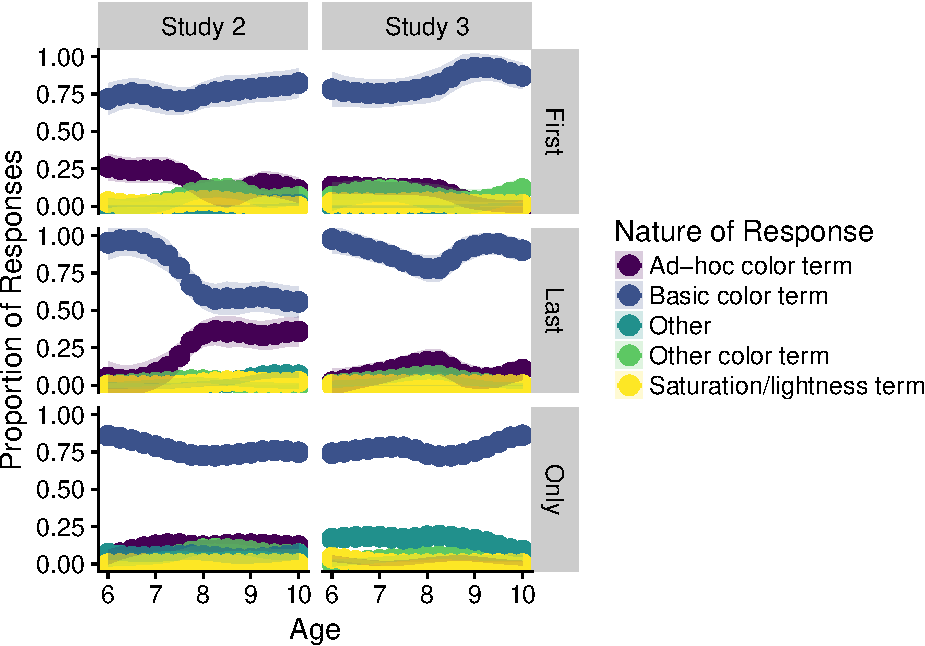
\includegraphics{amazon_color_files/figure-latex/crossstudy_accuracystrats-1.pdf}
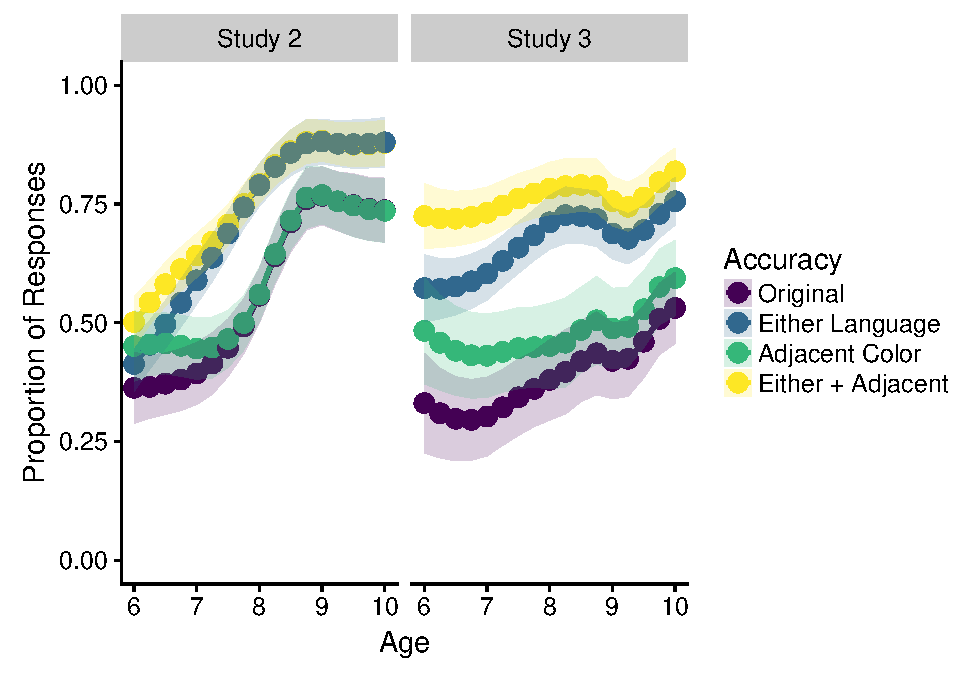
\includegraphics{amazon_color_files/figure-latex/crossstudy_accuracystrats-2.pdf}

\begin{figure}
\centering
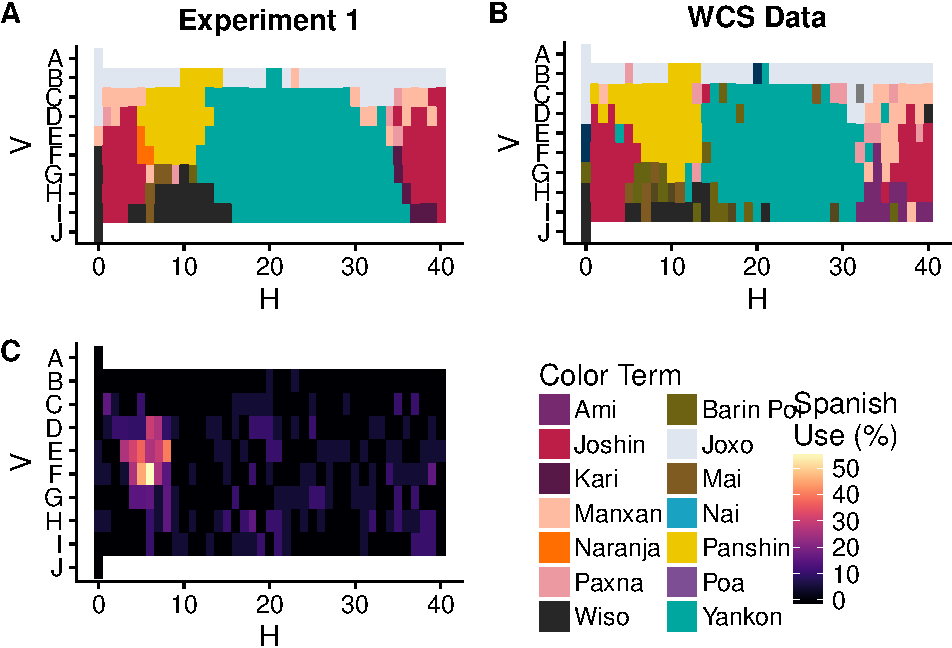
\includegraphics{amazon_color_files/figure-latex/adultfigure-1.pdf}
\caption{\label{fig:adultfigure}(A and B) Plots of the modal term given for
a particular chip. Color coordinates were represented in 2-D Munsell
space. Modal responses were given by SK adults during (A) the original
World Color Survey and during (B) our Study 1. (C) Heat map of
prevalence of Spanish-language responses during Study 1. Legends for all
three subplots located in the bottom-right quadrant.}
\end{figure}

\begin{verbatim}
## Warning: Column `prompt`/`Chip ID` joining factor and character vector,
## coercing into character vector
\end{verbatim}

\begin{verbatim}
## Warning: Removed 6 rows containing missing values (geom_smooth).
\end{verbatim}

\begin{figure}
\centering
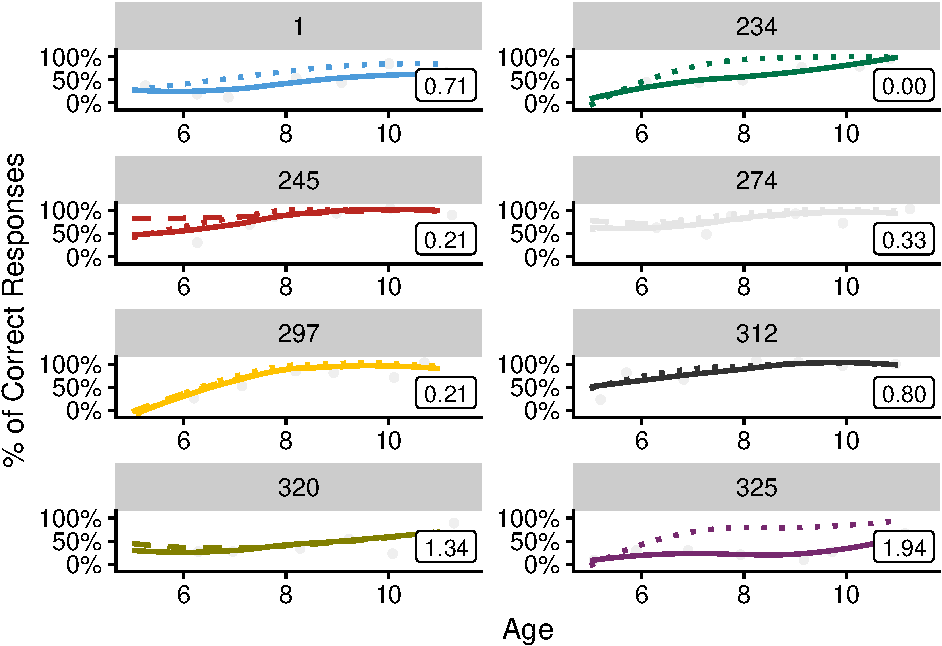
\includegraphics{amazon_color_files/figure-latex/childfigure-1.pdf}
\caption{\label{fig:childfigure}A comparison of children's performance
during the production task in Studies 2 and 3. Solid or dotted lines
represent overall performance by age for a particular chip. Solid lines
show whether the child gave a correct answer in the language indicated
in that column; dotted lines show if they gave a response that was
correct in either language. Line colors are representative of the chip's
color coordinates. Values in the lower-right corners of each subplot
display the entropy (uncertainty) values calculated from adult responses
given during Study 1.}
\end{figure}

\newpage

\section{References}\label{references}

\begingroup
\setlength{\parindent}{-0.5in} \setlength{\leftskip}{0.5in}

\hypertarget{refs}{}

\endgroup






\end{document}
